\documentclass[a4paper, notitlepage]{article}
\usepackage[english]{babel}
\usepackage[T1]{fontenc}
\usepackage[latin1]{inputenc}
\usepackage{amsfonts}
\usepackage{graphicx}
\usepackage{amssymb}
\usepackage{rotating}
\usepackage{amsthm}
\usepackage{amsmath}
\usepackage{amscd}
\usepackage{latexsym}
\usepackage{fancyhdr}
\usepackage{fancybox}
\usepackage{bbm}
\usepackage{fancybox}
\usepackage{enumitem}
\usepackage{natbib}
%\usepackage[%titleformat=italic,
%titleformat=commasep,
%commabeforerest,
%ibidem=strict,
%citefull=first,
%lookat,
%oxford,
%pages=format,
%idem%
%]{jurabib}
\usepackage{hyperref}
\usepackage{mathrsfs}
\usepackage{geometry}
\usepackage{dsfont}
\usepackage{picinpar}
\usepackage{tikz}
\usepackage{epstopdf}
\usepackage{url}
\usepackage{lastpage}
\usepackage{color}
\usepackage{verbatim}
\usepackage{float}
\usepackage[bottom]{footmisc}
\usepackage{attachfile}
\usepackage{listings} 
\usepackage[final]{pdfpages}
\usepackage{wasysym}
\usepackage{xfrac}
\usepackage{subfigure}
\usepackage{wrapfig}
\usepackage{sidecap}
%\usepackage{subfig}


%\geometry{left=2.0cm, right=2.0cm, top=3.0cm, bottom=3.0cm}
\DeclareGraphicsRule{.tif}{png}{.png}{`convert #1 `dirname #1`/`basename #1 .tif`.png}
\parindent0mm


\newcommand{\N}{\mathbbm{N}}
\newcommand{\Z}{\mathbbm{Z}}
\newcommand{\Q}{\mathbbm{Q}}
\newcommand{\R}{\mathbbm{R}}
\newcommand{\C}{\mathbbm{C}}
\newcommand{\E}{\mathbbm{1}}
\newcommand{\eps}{\varepsilon}
\renewcommand{\phi}{\varphi}
\newcommand{\epsgz}{$\varepsilon > 0$}
\newcommand{\impl}{\Rightarrow}
\newcommand{\aeq}{\Leftrightarrow}
\newcommand{\obda}{\emph{o.B.d.A.}}
\newcommand{\mvec}[2]{\left(\begin{matrix}#1\\#2\end{matrix}\right)}
\newcommand{\mvect}[3]{\left(\begin{matrix}#1\\#2\\#3\end{matrix}\right)}
\renewcommand{\qed}{\begin{flushright}\emph{(q.e.d.)}\end{flushright}}
\newcommand{\mustbe}{\stackrel{!}{=}}
\newcommand{\rg}{\mathrm{rg}}
\newcommand{\id}{\mathrm{id}}
\newcommand{\arsinh}{\mathrm{arsinh}}
\newcommand{\arcosh}{\mathrm{arcosh}}
\renewcommand{\l}{\left}
\renewcommand{\r}{\right}
\def\bi#1{\textbf{\em#1}}
\renewcommand{\d}{\mathrm{d}}
\newenvironment{alphenum}{\begin{enumerate}[label={(\alph*)}]}{\end{enumerate}}
\newenvironment{romenum}{\begin{enumerate}[label={(\roman*)}]}{\end{enumerate}}
\newenvironment{numenum}{\begin{enumerate}[label={\arabic*.}]}{\end{enumerate}}

\newcommand{\vecnormsq}[1]{\left|\left|#1\right|\right|_2}
\newcommand{\vecnorm}[1]{\left|\left|#1\right|\right|}


\lstset{numbers=left, 
		numberstyle=\tiny, 
		basicstyle=\footnotesize,
		numbersep=5pt,
		language=Python,
		keywordstyle=\color{blue},          % keyword style
  		commentstyle=\color{dkgreen},       % comment style
  		stringstyle=\color{mauve},         % string literal style
		} 
		
\lstset{extendedchars=\true}
\lstset{inputencoding=utf8}

\title{Miniproject: Robustness of storage capacity in more realistic Hopfield networks}
\author{Reinhold Bertram \\ 
Vince Moens \\ 	
{\it \large EPF Lausanne}\\
\vspace{0.5cm}\\
{\textbf{Assistant:} }\\
{Alex Seeholzer}\\
\\
{\textbf{Supervised by:}}\\
{Prof. Wulfram Gerstner, EPF Lausanne}
}
\date{\today}

\begin{filecontents}{ex2_lit_data}
#Perror 	pmax/N
0.001	0.105
0.0036	0.138
0.01		0.185
0.05		0.37
0.1		0.61
\end{filecontents}

\begin{document}

\maketitle
\thispagestyle{empty}
\vspace*{3 cm}

\begin{abstract}
In this report we will analyse how the storage capacity of a Hopfield Network changes when the Hebbian weight matrices is altered so that reciprocal connections are no longer symmetric. Furthermore Dale's law is considered, stating that synaptic connections to postsynaptic neurons are either of the excitatory or inhibitory type, never both. This makes the network more realistic.
\end{abstract}

\begin{figure}
\centering
\subfigure{
\includegraphics[width=0.2\textwidth]{EPFL_LOG_QUADRI_Red.eps}}
\end{figure}

\newpage
\pagenumbering{arabic}
\tableofcontents
\newpage

\section{Introduction}

Hopfield Networks were invented by John Hopfield in 1982 under the name of \textit{associative neural network}. They are content addressable binary memory systems that are used to model associative memory problems: 
\begin{quote}
\textit{Store a set of $p$ patterns $\psi_i^\mu$ in such a way that when presented with a new pattern $\zeta_i$, the network responds by producing whichever one of the stored patterns most closely resembles $\zeta_i$} \citep{Polk:2002fk}
\end{quote}

\begin{wrapfigure}{r}{6cm}
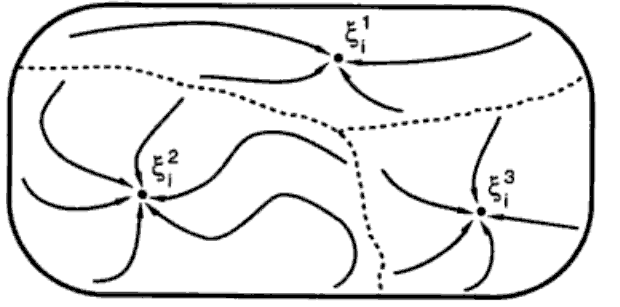
\includegraphics[width=6cm,angle=0]{PatternAttractors.png}
\caption{Configuration space showing the patterns as attractors}
\label{fig:PatternAttractors}
\end{wrapfigure}

In the configuration space of the network, the stored patterns $\psi_i^\mu$ act as attractors. While a Hopfield network is guaranteed to converge to a local minimum, convergence to one of the stored patterns is not a necessity. 

In order to facilitate the mathematical computation, the basis of the binary system is changed from a $\{0,1\}$ base to a $\{-1,1\}$ base.


\section{Exercise 1: Basic implementation of the Hopfield network}
\subsection{1.1 Getting started}

\begin{itshape}
\small
Asynchronous updating of the nodes ensures that the dynamics of the Hopfield model with symmetric weights $w_{ij} = w_{ji}$ always converge to a fixed point. An energy function in this case is given by:
\begin{equation}
H(t)=-\sum_{i=1}^n \sum_{j=1}^n \omega_{ij} S_i(t) S_j(t)
\label{eq: energy function}
\end{equation}
Implement the Hopfield network as described above. Shortly comment on your implementation. The overlap of the network in state $S(t)$ with a given pattern $\xi^{\mu}$ is defined by $\frac{1}{N}\sum_{i=1}^N \xi_i^{\mu} 	S_i(t)$. Set $N = 200$, $P = 5$, $c = 0.2$. For the first two unit time steps of the retrieval of one pattern, plot the changing values of the energy function and the overlap of the network with the pattern as the state of each node is sequentially updated.
\end{itshape}

\begin{wrapfigure}{r}{0.5\textwidth}
  \vspace{-20pt}
  \begin{center}
    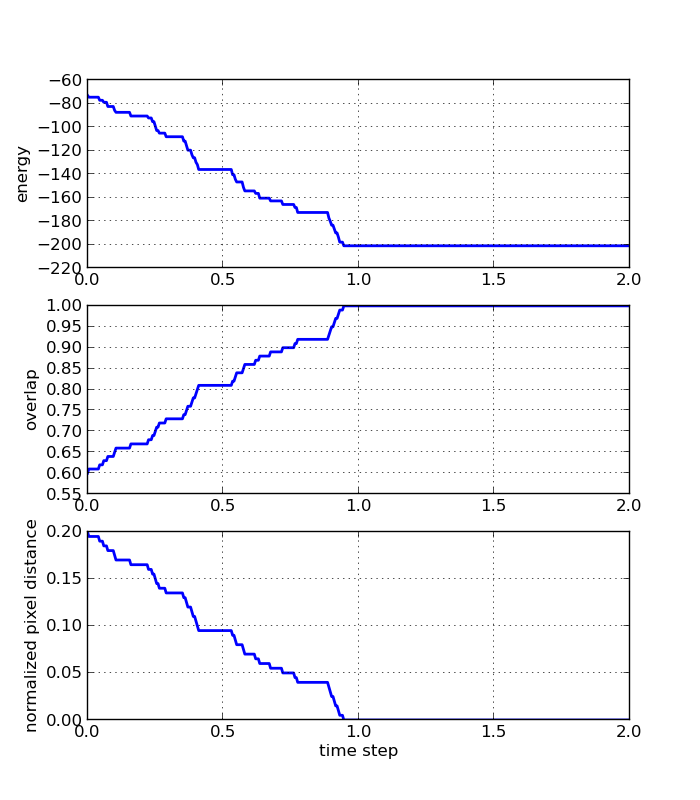
\includegraphics[width=0.48\textwidth]{dat/ex1_1-energy_overlap-N200-P5-c20}
  \end{center}
  \vspace{-20pt}
  \caption{Exercise 1	}
  \label{fig: Question 1.1}
  \vspace{-10pt}
\end{wrapfigure}

\paragraph*{}

The Hopfield Network was implemented and its source code can be found in the appendix.  In order to execute it, one should first execute \texttt{h=HopfieldNetwork()} in order  to initialize the class. Then one can execute the class using \texttt{h.run()}. The  options of the \texttt{run} function are \texttt{N} (number of pixels), \texttt{P}  (number of patterns), \texttt{ratio} (fraction of 1 in patterns), \texttt{mu} (pattern  chosen for retrieval), \texttt{flip$\_$ratio} (fraction of pixels that are to be  changed when creating the retrieval pattern), \texttt{pcut} (), \texttt{bPlot} (whether  a plot should be created) and \texttt{bDebug} (whether debugging tools should be turned  on).
By default the function is set to \texttt{run(self, N=200, P=5, ratio=0.5, mu=0,  flip$\_$ratio=0.2, pcut=0, bPlot=True, bDebug=False)}. 
At first, the script only ran very slowly, this is because we did not have a lot of  experience with python and thus used to for loops to do matrix multiplications. After  implementing the \texttt{numpy.dot} function, the script ran incredibly much faster. 

\subsection{1.2 Normalized Pixel Distance}
\begin{itshape}
\small
Using the overlap defined in 1.1, derive an expression for the percentage of pixels in the network state $S$ which differ from the pattern $\xi^\mu$. This is the (normalized) pixel distance.
\end{itshape}

\paragraph*{}

Since the overlap gives the fraction of pixels which are identical between the network in state $S(t)$ and the pattern $\xi^\mu$, and the normalized pixel distance must be normalized to the domain $[0,1]$, it must be given by:

\begin{equation}
d=\frac{1- \frac{1}{N} \sum_{i=1}^N \xi_i^{mu} S_i(t)}{2}
\end{equation}

The normalized pixel distance was plotted together with the energy and the overlap in figure \ref{fig: Question 1.1}.

\subsection{1.3 Pattern retrieval}

\begin{itshape}
\small
We define the retrieval error of a pattern $\xi^\mu$ in a Hopfield network as the normalized pixel distance of the network state $S$ to the pattern $\xi^\mu$ after convergence, when retrieving the pattern $\xi^\mu$ as described above.

Set N = 200 and c = 0.1. Plot the mean retrieval error of a randomly chosen pattern averaged over different network realizations as a function of the dictionary size P. Average over enough network realizations to give a smooth curve and give error bars for the estimation of the mean (you can assume the variation to be normally distributed). From your data points and the chosen confidence interval, roughly estimate a maximal P at which patterns can be retrieved from the network with a mean retrieval error of less than 2$\%$?

\end{itshape}

\begin{wrapfigure}{r}{0.5\textwidth}
  \vspace{-20pt}
  \begin{center}
    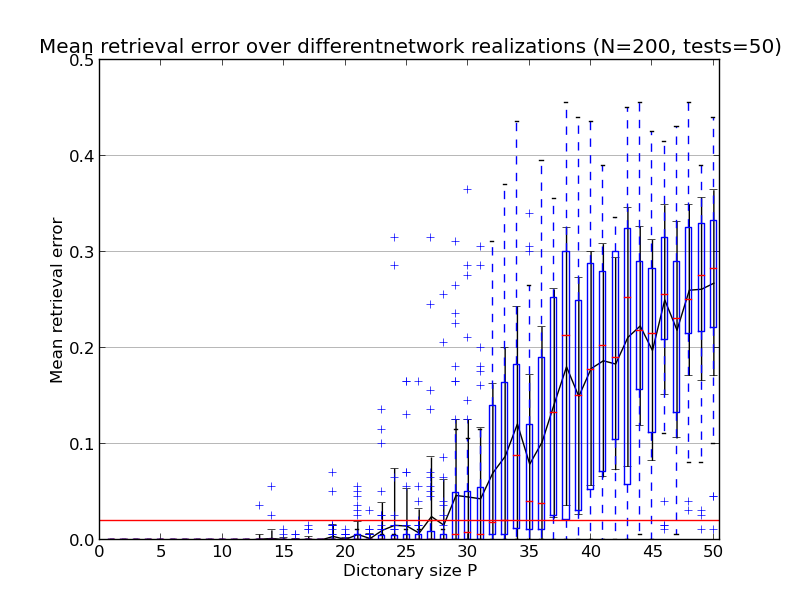
\includegraphics[width=0.6\textwidth]{dat/ex1_3-error_avg-N200-P50-Q50.png}
  \end{center}
  \vspace{-20pt}
  \caption{Exercise 1.3: Mean retrieval error averaged over 100 different network realizations.}
  \label{fig: Question 1.3}
  \vspace{-10pt}
\end{wrapfigure}

\paragraph*{}

Figure \ref{fig: Question 1.3} shows a plot of the mean retrieval error with respect to the dictionary size P. As one can see, the error remains very close to 0 for a dictionary size lower than 20. After that the error starts increasing. We have included a horizontal line at y = 0.02 indicating the 2$\%$ error. From that line, one would roughly estimate that the maximal P at which patterns can be retrieved is P=35. 


\section{Exercise 2: Capacity estimation}

\begin{itshape}
\small
We now define the capacity of a Hopfield network of size N as the number of patterns $P_{N,max}$ that can be stored, such that the mean retrieval error averaged over all stored patterns (one retrieval attempt each) is at most 2$\%$. This yields the maximal load $\alpha_{N,max} = \frac{P_{N,max} }{N}$.

Set c=0.1. Calculate $\alpha_{N,max}$ for at least 10 network realizations and state the mean together with confidence intervals. Do this for N = 100, 250 and one other larger network size. Shortly interpret the resulting values and compare with results from literature.
\end{itshape}

\paragraph*{}


%\begin{table}[H] 
\centering 
\begin{tabular}{|l|l|l|l|l|l|l|} 
\hline 
N & tests & C-level & maximal load & lower bound & upper bound & $P_{N,max}$\\ 
 \hline \hline 
100 & 10 & 95.0 $ \% $& 0.1180 & 0.1163 & 0.1197 & 11.80 \\ 
250 & 10 & 95.0 $ \% $& 0.1252 & 0.1246 & 0.1258 & 31.30 \\ 
500 & 10 & 95.0 $ \% $& 0.1282 & 0.1279 & 0.1285 & 64.10 \\ 
\hline 
\end{tabular} 
\end{table} 



\section{Exercise 3: Random asymmetry}

\begin{itshape}
\small
To investigate the robustness of pattern retrieval against asymmetry in the weight matrix, consider now networks where for each pairs of nodes $\l(i, j\r)$, the directed connection from node $i$ to node $j$ is cut with probability $p_{cut}$. This will introduce asymmetry in the Hebbian weight matrix Eq. 1.

Set $c=0.1$ and $N = 200$. As in Ex. 2 calculate and plot the mean $\alpha_{N,max}$ for varying $p_{cut}$ with error bars (at least 10 repetitions). At which $p_{cut}$ does the maximal load drop below $50\%$ of the value estimated in Ex. 2? State the confidence interval.

Note: Bare in mind that the convergence assertion of Question 1.1 does not necessarily hold for $p_{cut} > 0$.
\end{itshape}

\paragraph*{}



\begin{wrapfigure}{r}{0.5\textwidth}
  \vspace{-20pt}
  \begin{center}
    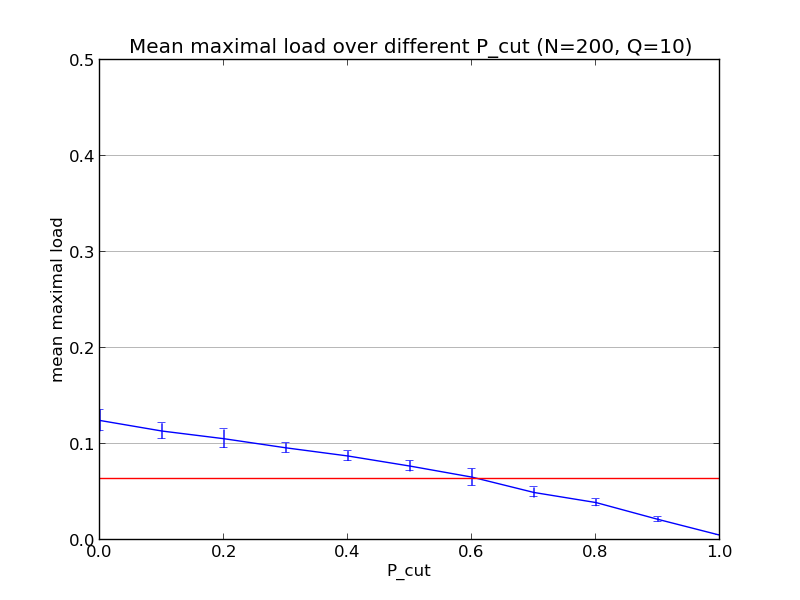
\includegraphics[width=0.6\textwidth]{dat/ex3-mean_max_load-N200-Q10-C95}
  \end{center}
  \vspace{-20pt}
  \caption{Exercise 3: Maximal load $\alpha_{N,max}$ averaged over 10 repetitions for varying $p_{cut}$ }
  \label{fig:exercise3}
  \vspace{-10pt}
\end{wrapfigure}

Figure \ref{fig:exercise3} shows the the $\alpha_{N,max}$ over varying $p_{cut}$.

With increasing $p_{cut}$ the maximal load decreases. At $p_{cut} = xxx$ the maximal load drops below $\50%$ of the value estimated in exercise 2.

\section{Exercise 4: Dale's law}

\begin{itshape}
\small
Set $c=0.1$, $N = 200$ and turn off random asymmetry ($p_{cut} = 0$). Set $E \in \l[0, 1\r]$ to be the percentage of excitatory nodes.

For a given $E$, randomly split the network into an excitatory and an inhibitory subpopulation (of sizes $E \cdot N$ and $(1 - E) \cdot N$ respectively). Now enforce Dale's law on the network connectivity by setting '"disallowed"` connection weights in the standard Hebbian weight matrix Eq. 1 to zero.

What percentage of the directed connections do you expect to be cut for $E = \frac{1}{2}$
As in Ex. 2 calculate and plot the mean $\alpha_{N,max}$ for varying E with error bars (at least 10 repetitions). Interpret the results and compare the value for E = 1 to your result from Ex. 3.
\end{itshape}

\paragraph*{}

\begin{wrapfigure}{r}{0.5\textwidth}
  \vspace{-20pt}
  \begin{center}
    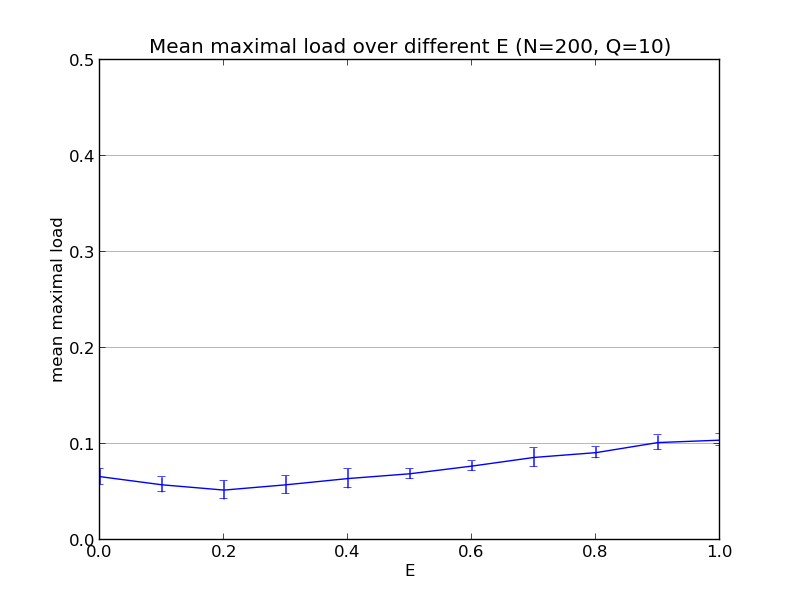
\includegraphics[width=0.6\textwidth]{dat/ex4-mean_max_load-N200-Q10-C95.png}
  \end{center}
  \vspace{-20pt}
  \caption{Exercise 4: Mean maximal load over different E}
  \label{fig: Question 1.3}
  \vspace{-10pt}
\end{wrapfigure}



\section{Conclusion}




\nocite*{}
%\addcontentsline{toc}{section}{References}
\bibliographystyle{alpha}
\bibliography{bibliography}

\newpage

%\section{Appendix}
\subsection{Code of Hopfield Network}
\label{ssec: Hopfield Network}
\lstinputlisting[frame=single,caption=hopfield.py]{../src/hopfield.py}
\newpage
\subsection{Code of exercise 1:}
\lstinputlisting[frame=single,caption=exercise1\_1.py]{../src/exercise1_1.py}
\lstinputlisting[frame=single,caption=exercise1\_3.py]{../src/exercise1_3.py}
\newpage
\subsection{Code of exercise 2:}
\lstinputlisting[frame=single,caption=exercise2.py]{../src/exercise2.py}
\newpage
\subsection{Code of exercise 3:}
\lstinputlisting[frame=single,caption=exercise3.py]{../src/exercise3.py}
\newpage
\subsection{Code of exercise 4:}
\lstinputlisting[frame=single,caption=exercise4.py]{../src/exercise4.py}

\end{document}
